Before going deep into structural properties of decomposable digraphs we first need to establish what a graph is.
For some graph $G(V,E)$ where $V$ and $E$ are two sets contaning the vertices (also commonly called nodes) and egdes of the graph respectivlely.
%Example $V=\lbrace a,b,c \rbrace$ then $a,\ b$ and $c$ are three distinct vertices of the graph $G$ and the only vertices of $G$.
We define the \textbf{size} of the graph to be the number of vertices $|V|$ this is also known as \textbf{cardinality} of $V$.
%In the case of the example the size of $G$ $|V|=3$ it is also called the order of a graph.
An \textbf{edge} $e \in E$ where $e \equiv (a, b)$ and $\{ a, b \} \subseteq V$ then $e$ is an edge in $G$, $e$ is said to be \textbf{incedent} to $a$ and $b$. 
We call $a,b \in V$ \textbf{adjecent} if there is an edge $(a,b)$ or $(b,a)$ (an edge between the two given vertices is said to be adjecent).
If an edge goes from and to the same vertex $(a,a)$ it is called a \textbf{loop}.
The set of edges $e_1, \dots, e_k$ is usally describe whit the letter $E$ where each edge contains a pair of vertices that are adjecent. \\
In a graph we have something called a \textbf{walk} which is a alternately ordering of vertices an edges in the graph $G$ where the edge in between the two vertices in the ordering is an edge between the vertices in $G$ (for $(a,e_1,b)$ to be a walk the edge $e_1$ has to be between $a$ and $b$).
We call a walk closed if the first vertex in the walk is the same as the last.\\
Every vertex $v\in V$ of $G(V,E)$ have a \textbf{degree} denoted $d(v)$ which is the number of incident edges to $v$.
A \textbf{path} in a graph is a walk where each vertex in the ordering can only apear one time. A cycle is a closed walk where the only vertex pressent more then one time is the first vertex(for the walk to be closed the first vertex has to apear last to also called a closed path).
Let $X$ be a subset of the vertices $X\subseteq V$ then we say that $V\backslash X$ is the set of vertices with out the vertices in $X$, i.e. $V/X \equiv V-X$. 
A subgraph $H$ of $G$ can contain any of the vertices and the arcs connected to the chossen vertecies in H. you can not have an edge conecting no vertices in $H$ but you do not have to choose all the arcs in $G$ between the chossen vertices in $H$ for $H$ being a subgraph. 
%The describe example can be seen in figure \autoref{fig:graph}.
\begin{figure}[!h]
    \begin{subfigure}{0.48\textwidth}
        \centering
        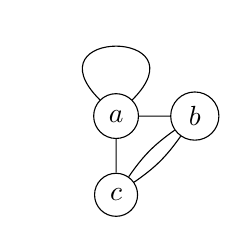
\begin{tikzpicture}
            [main/.style ={draw,circle}]
            \node[main] (a){$a$};
            \node[main] (b)[right of = a]{$b$};
            \node[main](c)[below of= a]{$c$};
            \draw (a) to (b) (c) to (a) (c) to [bend right =10](b) (c) to [bend left =10](b); 
            \draw (a) to [loop,red] (a);
        \end{tikzpicture} 
        \caption{graph $G(V,E)$ is an example of a graphs, the red edge is a loop, and all pair of vertices in this graph is adjecent.}
        \label{fig:graph}
    \end{subfigure}
   \begin{subfigure}{0.48\textwidth}
    \centering
        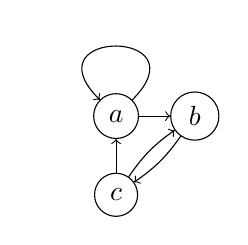
\begin{tikzpicture}
            [main/.style ={draw,circle}]
            \node[main] (a){$a$};
            \node[main] (b)[right of = a]{$b$};
            \node[main](c)[below of= a]{$c$};
            \draw[->] (a) to (b);
            \draw[->](c) to (a);
            \draw[->](c) to [bend left =10](b);
            \draw[->](b) to [bend left =10](c); 
            \draw[->] (a) to [loop,red] (a);
        \end{tikzpicture} 
        \caption{This is an oriantation of the edges in the graph which makes this a digraph}
        \label{fig:digraph}
   \end{subfigure}
\end{figure}


Before delving more specific into graphs and digraphs we must establish some important prerequisite and properties. 
A graph is called \textbf{simple} if there is no loops and no multiple edges. 
With multiple edges it means multiple edges between the same pair of vertices like in \autoref{fig:graph} between $b$ and $c$.
\begin{figure}[!h]
	\centering
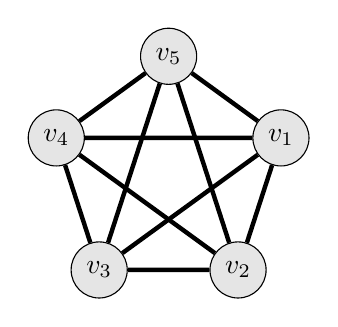
\begin{tikzpicture}[
	xs/.style = {xshift=#1 mm},
	ys/.style = {yshift=#1 mm}]
	
	\def \n {5}
	\def \radius {1.5cm}
	\def \margin {8} % margin in angles, depends on the radius
	
	\foreach \s in {1,...,\n}
	{
		\node[draw, circle][fill=gray!20!white] (\s) at ({360/\n * -(\s+3.75)}:\radius) {$v_\s$};
	}
    \draw[ultra thick] (1) -- (2) (1) -- (3) (1) -- (4) (1) -- (5);
    \draw[ultra thick] (2) -- (3) (2) -- (4) (2) -- (5);
    \draw[ultra thick] (3) -- (4) (3) -- (5);
    \draw[ultra thick] (4) -- (5);
    \end{tikzpicture}
\caption{Complete graph with 5 vertices.}
\label{fig:complete}
\end{figure}

A graph is \textbf{connected} if there exists a path between all pair of vertices in the graph and \textbf{disconnected} otherwise.
A graph is called \textbf{complete} if there for all pair of vertices in the graph is an edge between them see \autoref{fig:complete}.\\

If we instead of edges have \textbf{arcs} between the vertices we call it a \textbf{digraph}.
An arc is describe just like an egde with two adjecent vertices $(a,b)$ the first vertex mentioned in an arc is the vertex \textbf{from} where the arc starts also called the \textbf{tail}, the second vertex is where the arc is pointing \textbf{to} also called \textbf{head}. The set of arcs is normaly denoted $A$ like the set of edges is denoted $E$. 
So the arc $(a,b)$ goes from $a$ to $b$, if you wanted it the other way around the arc is $(b,a)$.
These graph contaning only arcs and no edges is called a digraph $G(V,A)$ which is what we in this project are focusing on see \autoref{fig:digraph}.\\
For two vertices $x$ and $y$ in $D(V,A)$ then if we have an arc from $x$ to $y$ we say that $x$ \textbf{dominates} $y$ this is denoted like this $x \rightarrow y$. If we talk about subgraphs $A$ and $B$, then $A$ \textbf{dominates} $B$ if for all $a\in A$ and $b,\in B$, $a \rightarrow b$. If there is no arcs from $B$ to $A$ we denote it $A\mapsto B$ and if both $A\rightarrow B$ and $A \mapsto B$ we say that $A$ \textbf{completely dominates} $B$ and this is denoted $A\Rightarrow B$. 

In a digraph we have something called the \textbf{underlying graph}. 
An underlying graph of a digraph is where all arcs are replaced by edges (edge is used every time we talk about undirected edges between vertices, when using directions it is called an arc).
Let $X \subseteq V$ Then we can make the subdigraph $D\left< X\right>$ which is the subgraph $D$ induced by the set $X$ meaning that all the vertices is from $X$ and the arcs is from $A\in G$ but where both head and tail is incedent to the vertices in $X$. We will denote the graph $D\left< V\backslash X\right>$ for some $X\subseteq V$ as $D-X$.
A digraph is \textbf{connected} if the underlying graph is connected, (also called weakly connected), a digraph can be \textbf{strongly connected} and \textbf{semi connected} too.
A digraph is called \textbf{semi connected} if there for each pair $u$ and $v$ exists a path from either $u$ to $v$ or $v$.  
It is said to be \textbf{strongly connected} if for each pair of vertices $u$ and $v$ there exists a path from both $u$ to $v$ and $v$ to $u$. A strongly connected digraph is also called a \textbf{strong} digraph. 
A strong digraph have a subset $S$ called a \textbf{seperator} if $D-S$ is not strong, we also say that $S$ \textbf{seperates} $D$. 
A seperator $S$ is called \textbf{minimal seperator} of $D$ if there exists no proper subset $X\subset S$ that seperates $D$.
Now we can introduce a \textbf{$k$-strong} digraph $D$ which is a strong digraph with $|V|\geq k+1$ and a minimal seperator $S$ \textcolor{red}{on} $|S|\geq k$.

In a digraph $D(V,A)$ we mostly use the \textbf{dregree} as two different degrees namely \textbf{out degree}, $d^+(v)$,and \textbf{in degree}, $d^-(v)$, that is the arcs from $v$ and to $v$ respectively.








\section{somthing else}
We can use \textcolor{red}{these} to describe som specific collection of graphs as the graph \textbf{tournaments}.
\textbf{Tournaments} is a digraph where the underlying graph is complete. 
So a complete graph of order 5 any orientation of the edges concludes in a tournament.
If instead of replacing the one edge by one arc in either direction, but instead replace it by two arcs the digraph is called \textbf{semicomplete}.

The reason for grouping the digraphs into smaller collections of digraphs (like tournaments is a smaller collection of semicomplete digraphs) is because of problems that is hard to solve on general graph but is easy/polynomial solvable on specific graphs.

A group of these problems is called NP-hard problems which sometimes sound easy solvable for graphs but only for some specific graphs we know how to solve it in polynomial time. 
\begin{definition}
    define NP-hard problems
\end{definition}

\textcolor{red}{In this paper we focusing on the specific digraphs that are \textbf{decomposable}. 
A \textbf{decomposable} digraph is a digraph $D=H[G_1,G_2,\dots,G_|H|]$ where each $G_i$ is sconnected graphs replacing each vertex of the digraph $H$.} ...
